\documentclass[conference]{IEEEtran}
\IEEEoverridecommandlockouts
\usepackage{cite}
\usepackage{amsmath,amssymb,amsfonts}
\usepackage{algorithmic}
\usepackage{graphicx}
\usepackage{textcomp}
\usepackage{xcolor}
\usepackage{booktabs}
\usepackage{pifont}
\usepackage{tikz}
\usetikzlibrary{positioning}
\usepackage{pgfplots}
\pgfplotsset{compat=1.16}
\usepackage[T1]{fontenc}
\usepackage[utf8]{inputenc}
\usepackage{url}
\def\BibTeX{{\rm B\kern-.05em{\sc i\kern-.025em b}\kern-.08em
    T\kern-.1667em\lower.7ex\hbox{E}\kern-.125emX}}
\newcommand{\code}[1]{\texttt{#1}}

\begin{document}

\title{XS3: A Spec-Free, Machine-Exact Triple-Graph\\Notation for LLM-to-LLM Communication}

\author{\IEEEauthorblockN{V\~u V\u{a}n Minh Quang}
\IEEEauthorblockA{\textit{VDG Solutions} \\
Archived: Zenodo concept DOI \texttt{10.5281/zenodo.21425813}}}

\maketitle

\begin{abstract}
Large language models increasingly communicate with one another---across
compaction boundaries, agent hand-offs, and tool pipelines---yet they still
exchange state as free prose, which paraphrases and silently corrupts facts.
We present XS3, a controlled notation in which \emph{one sentence is exactly one
labeled graph edge} (\code{subject predicate object .}). A document \emph{is}
its edge set; a small, fixed glyph vocabulary desugars mechanically into
reified edges, so every well-formed document decodes to a unique triple graph.
Two properties distinguish XS3. First, \emph{spec-free comprehension}: because
each token is chosen to be the strongest natural key for the concept region it
activates in a pre-trained model, a language model reads XS3 correctly with no
grammar, glossary, or specification supplied in context; we validate this across
model families with blind cold reads. Second, \emph{machine exactness}: a
dependency-free reference decoder round-trips every construct through a canonical
serialization (decode $\rightarrow$ serialize $\rightarrow$ decode is edge-exact
and idempotent), passing $5000/5000$ generated documents. We report an iconicity
study of glyph choice that led us to replace an overloaded negation marker with
the universal mathematical~$\neg$, and a compaction study showing that, under a
fixed budget, accumulated XS3 state degrades by \emph{visible omission} of whole
edges while equivalent prose degrades by \emph{silent corruption}. We argue that
XS3's value is not token compression but corruption-resistant, addressable state.
\end{abstract}

\begin{IEEEkeywords}
controlled natural language, knowledge representation, triple graph, agent
communication, large language models, constrained decoding, context compaction
\end{IEEEkeywords}

\section{Introduction}
Autonomous agents built on large language models (LLMs) rarely operate in a
single, unbroken context. State crosses \emph{compaction} boundaries when a
conversation is summarized to fit a window; it crosses \emph{hand-offs} when one
agent briefs another; it crosses \emph{tool} boundaries when structured facts are
serialized and re-read. At each crossing the medium is almost always free prose,
and prose is lossy under paraphrase: a fact is re-worded, a qualifier is
dropped, a number is smoothed, and---crucially---the reader cannot tell that a
plausible-looking sentence is now wrong.

We ask a narrower question than ``how should agents talk in general.'' We ask:
\emph{what notation lets one model write state that another model reads back
without drift, using only knowledge both models already have?} Our answer, XS3,
makes three commitments:

\begin{enumerate}
\item \textbf{One sentence, one edge.} Every sentence \code{s p o .} is a single
labeled, directed edge. A document is a \emph{set} of edges; sentence order
carries no meaning except inside an explicit ordered sequence \code{< >}. All
metadata (time, degree, negation, deontics, provenance) is \emph{reified}: it
becomes edges about edges, so the document is always a plain graph.
\item \textbf{Comprehension before parsing.} The primary correctness criterion is
whether a specification-free model reads a snippet correctly, not whether a strict
parser accepts it. Glyphs and core vocabulary are chosen to be the strongest
\emph{natural keys} for the regions they activate in a pre-trained model.
\item \textbf{Exactness through structure.} Machine determinism rides a canonical
serialization of the graph, not a natural-language readback. Decoding is exact;
the English render is a best-effort human view.
\end{enumerate}

This paper describes the design (Sec.~\ref{sec:design}--\ref{sec:lang}), the
exactness mechanism and its test harness (Sec.~\ref{sec:exact}), a comprehension
and glyph-iconicity evaluation (Sec.~\ref{sec:comp}), and an application to
accumulated agent state and context compaction (Sec.~\ref{sec:compact}), where
XS3's corruption-resistance is most visible.

\section{Design Principles}\label{sec:design}

\subsection{The document is a graph}
Let $G=(V,E)$ be a directed, edge-labeled multigraph. An XS3 sentence
\code{s p o .} contributes one edge $(s,p,o)$. Chaining is purely syntactic
sugar over the same edge set: \code{;} keeps the subject and switches predicate,
\code{,} keeps subject and predicate and adds an object. Thus
\code{an age 30; job dev.} $\equiv$ \code{\{(an,age,30),(an,job,dev)\}}.
Because a document is a set, two independently written documents that denote the
same graph normalize to the same canonical form and hash---an order-invariance
that prose does not possess.

\subsection{Reification keeps everything monotone}
A plain triple graph is monotone and existential-positive: it can only assert
that edges are present. Anything that is not a positive fact---time, strength,
modality, negation, rationale---is expressed by \emph{reifying} the target edge
into a node and attaching a further edge to it. A qualifier is sugar for this:
\code{s p o @2020} desugars to \code{\{s p o\} at 2020}; \code{s p o \%80} to
\code{\{s p o\} deg 80}. Reification is what lets a notation with negation and
modality still decode to a single, plain edge set.

\subsection{Comprehension-first and the natural-key rule}\label{sec:key}
An LLM already carries, from pre-training, representations for ``inverse
relation,'' ``negation,'' ``prohibition,'' ``time,'' and so on. XS3 treats a
glyph as a \emph{retrieval key} into those representations. The design rule is:
each token must be the strongest natural key for the region it names. A token
that is not a natural key \emph{sinks}---the model reads past it. We found this
empirically (Sec.~\ref{sec:comp}): a degree-zero marker pressed into service as
negation was read as ``degree zero,'' not ``not,'' and had to be replaced.

A corollary is a boundary on what XS3 should invent. Structural glyphs are drawn
from conventions every model has seen: mathematics ($\neg$, $\Rightarrow$,
$=$, $\in$), code (\code{?}, \code{\#}, \code{\{\}}, \code{<>}), and ordinary
English content words. Domain vocabulary is open Unicode---an author may write
predicates and entities in any language---so XS3 is not English-only; only a
small closed set of logical/structural keywords is fixed.

\section{The Language}\label{sec:lang}

\subsection{Glyphs}
The structural glyphs are: \code{.} (end sentence), \code{;} and \code{,}
(chaining), \code{\#x} (anchor: same name, same node), \code{?x} (variable, legal
only inside \code{\{\}}), \code{\^{}p} (inverse predicate), \code{\{\}} (a
subgraph as one node---a world, belief, plan, or rule body), \code{[s p o]}
(an edge \emph{mention}, referenced without assertion), \code{< >} (the only
ordered construct), \code{"\dots"} (opaque string), and \code{//} (comment).
Three attention-anchor qualifiers ride an asserted edge---\code{@} time,
\code{\%} degree, and \code{!} a salient operator marker for engine pragmas
(\code{!must}, \code{!physics}) and prohibition (\code{!\ding{55}}).

\subsection{Negation as a universal prefix}
Logical negation is written with the mathematical~$\neg$ as a prefix on
\emph{one} predicate (\code{s $\neg$p o}) or on \emph{one} edge mention
(\code{$\neg$[s p o]}). It desugars to a single meta-edge stating that the
edge does not hold, and the positive triple is never emitted:
\[
\text{\code{an $\neg$love bao}} \;\longrightarrow\; \{(\,[an\;love\;bao],\ \text{mark},\ \text{not}\,)\}.
\]
Negation is deliberately restricted to a single edge. A negated conjunction
\code{$\neg$\{A; B; C\}} is forbidden because, by De~Morgan's law, it denotes
$\neg A \vee \neg B \vee \neg C$; disjunction has no image in a monotone edge set
and would break the graph invariant. To deny several edges, one negates each.

\subsection{Self-description}
From its second line onward the language card is written in XS3 and defines XS3;
each line is simultaneously a rule and a live example of itself. This is possible
precisely because the notation is spec-free to read: a model can consume the
self-definition without a prior grammar.

\begin{figure}[t]
\centering
\fbox{\begin{minipage}{0.88\columnwidth}
\small\ttfamily
\#deploy a policy; owner platform.\\
you run tests !must.\\
prod $\neg$has feature-flags.\\
\{tests pass\} =\textgreater\ \{you tag release !must\}.
\end{minipage}}
\caption{A small XS3 document. It decodes to six edges: two assert facts about
\texttt{\#deploy}; \texttt{!must} reifies onto its edge as
\texttt{[you run tests] mark must}; \texttt{$\neg$has} emits \emph{only} the
negation meta-edge \texttt{[prod has feature-flags] mark not} and never the
positive triple; and the rule \texttt{=\textgreater} relates two subgraph nodes.
Order is irrelevant: any permutation denotes the same graph.}
\label{fig:example}
\end{figure}

\begin{table}[t]
\caption{Qualifier and negation desugaring; each surface form is a graph equation.}
\label{tab:desugar}
\centering\small
\begin{tabular}{@{}ll@{}}
\toprule
Surface form & Reified edge(s) \\
\midrule
\texttt{s p o @t}    & \texttt{\{s p o\} at t} \\
\texttt{s p o \%n}   & \texttt{\{s p o\} deg n} \\
\texttt{s p o !m}    & \texttt{[s p o] mark m} \\
\texttt{s $\neg$p o} & \texttt{[s p o] mark not} \quad(positive triple absent) \\
\bottomrule
\end{tabular}
\end{table}

\section{Machine Exactness}\label{sec:exact}
Human readback (graph $\rightarrow$ English) is inherently lossy and is treated
as non-normative. Machine exactness instead rides a \emph{structural} canonical
form. The reference decoder \code{E$_0$} implements three operations:
\emph{decode} (XS3 $\rightarrow$ edge set), \emph{serialize} (edge set
$\rightarrow$ canonical XS3), and a best-effort \emph{readback} (edge set
$\rightarrow$ English). The correctness contract is, for every document $d$,
\[
\text{decode}(\text{serialize}(\text{decode}(d))) \;=\; \text{decode}(d),
\]
together with idempotence of \code{serialize}$\,\circ\,$\code{decode}. A property
test generates random documents spanning all constructs (chaining, anchors,
sequences, rules, reified qualifiers, negation, deontics) and checks edge-set
equality and idempotence. The current harness passes $5000/5000$ documents with
zero parse, round-trip, or idempotence failures; the informational
English-readback rate is $1.0$ on the same corpus. Because negation and other
qualifiers desugar to ordinary meta-edges, adding the $\neg$ prefix required no
change to the edge-equality contract: a document written with $\neg$ and one
written with the legacy marker denote the same edge set.

\section{Comprehension and Iconicity}\label{sec:comp}

\begin{table}[t]
\caption{Summary of the nine empirical studies (\S\ref{sec:exact}--\S\ref{sec:compact}).}
\label{tab:studies}
\centering\small
\begin{tabular}{@{}cp{6.6cm}@{}}
\toprule
\# & Study and headline result \\
\midrule
S1 & Spec-free cold comprehension: models recover steps, rules, and deontics from XS3 with no grammar in context \\
S2 & Negation iconicity ($\%0\!\to\!$\code{!not}$\to\neg$): $\neg$ read as negation in $4/4$ mixed tests; \code{!} polysemy removed \\
S3 & Glyph audit: $\sim$ weak (model self-reports uncertainty), $\%$ and $\neg$ strong \\
S4 & Deontic verb-anchoring: a bare-noun marker leaks polarity; a verb-anchored clause reads correctly \\
S5 & Self-reference: the prior marker collides in metalanguage; a \code{//} comment or explicit $\neg$ reads correctly \\
S6 & Structural round-trip: $5000/5000$, English rate $1.0$ \\
S7 & Budgeted compaction: XS3 $13/18$ exact ($2$ wrong) vs.\ prose $2/18$ exact ($10$ silently wrong) \\
S8 & Edge-aging prototype: $10/10$ pinned exact; $73\%$ smaller than un-aged; bounded live set \\
S9 & Salience selection: LLM keeps $6/6$ critical facts; a recency policy $0/6$ \\
\bottomrule
\end{tabular}
\end{table}

We evaluate the comprehension-first thesis with \emph{blind cold reads}: a model
is given only an XS3 snippet and neutral questions, with no card, glossary, or
grammar in context, and asked to reconstruct the facts. Across model families and
tiers, models recover ordered steps, conditional rules, reified qualifiers, and
deontics from XS3 alone. This is a claim about semantics, not surface: the
operators map onto textbook graph, set, and relational-algebra notions
(converse~$\code{\^{}}$, quotient~$=$, closure~$\Rightarrow$, membership~$\in$)
that every model has seen.

\subsection{An iconicity study of negation}
The natural-key rule (Sec.~\ref{sec:key}) is not a priori; it is forced by data.
We iterated the negation marker three times.
\begin{itemize}
\item \textbf{Degree-zero (\code{\%0}).} Read as ``degree zero,'' never as
negation---the marker sank. Rejected.
\item \textbf{Salient word (\code{!not}).} Read correctly in \emph{action}
clauses, but it overloaded the \code{!} operator: with negation living on
\code{!}, models intermittently re-read \code{!must} as ``not must'' (optional).
It also failed under self-reference: a clause \emph{about} the glyph
(\code{\%0 means negation !not}) was read as ``\%0 \emph{is} negation.''
\item \textbf{Universal $\neg$.} A prefix drawn from mathematics. In blind
mixed-modality tests---documents interleaving $\neg$ with \code{!must} and
\code{!\ding{55}}---every model classified $\neg$ clauses as negated facts,
\code{!must} as mandatory, and explicitly reported that ``\code{!} is not
negation.'' The polysemy vanished because $\neg$ carries its own strong prior and
no longer leans on \code{!}.
\end{itemize}
A control finding sharpened the rule: a superficially similar bracketed marker
that was \emph{not} a standard symbol reintroduced the overload, whereas $\neg$
did not---confirming that the win comes from \emph{universality of the
convention}, not from separating negation \emph{per se}. A parallel audit retired
an affect qualifier whose glyph a model self-reported as ``inferring from
pattern, not certain,'' in favor of an ordinary predicate.

\subsection{Writing rules}
Two writing rules emerged from the same method. Deontic markers must bind a
\emph{verb-anchored} clause (\code{you force dom !\ding{55}}), never a bare noun,
which leaks its polarity. And self-referential statements about XS3's own glyphs
are commentary, not domain facts: they are best written as a \code{//} comment or
plain prose, or, if they must be queryable, with an explicit $\neg$ over a quoted
mention.

\section{Application: Accumulated State and Compaction}\label{sec:compact}
The sharpest use of XS3 is as \emph{running state} that survives repeated
re-summarization. Here the correct operation is not ``rewrite more concisely''
but \emph{stack and dedup}: copy existing edges verbatim, append new ones, and
drop only exact duplicates. Because edges are atomic and addressable, an old fact
either survives byte-identical or is dropped as a whole edge; it is never
paraphrased into a subtly wrong sentence.

\subsection{A budgeted-compaction experiment}
We accumulated eighteen checkable facts (DOIs, commit hashes, glyph rules,
counts) into a running state under a fixed token budget that forced roughly half
to be shed, comparing two arms with identical instructions and facts: one
carrying state as prose, one as XS3 edges. A blind grader then scored each of the
eighteen facts in each arm as \emph{fully retained}, \emph{lost}, or
\emph{wrong} (stated but corrupted). Table~\ref{tab:drift} summarizes the outcome.

\begin{table}[t]
\caption{Fact retention after budgeted compaction (18 facts).}
\label{tab:drift}
\centering
\begin{tabular}{lccc}
\toprule
State medium & Fully retained & Lost & \textbf{Wrong (silent)} \\
\midrule
Prose        & 2  & 6 & \textbf{10} \\
XS3 edges    & 13 & 3 & \textbf{2} \\
\bottomrule
\end{tabular}
\end{table}

\begin{figure}[t]
\centering
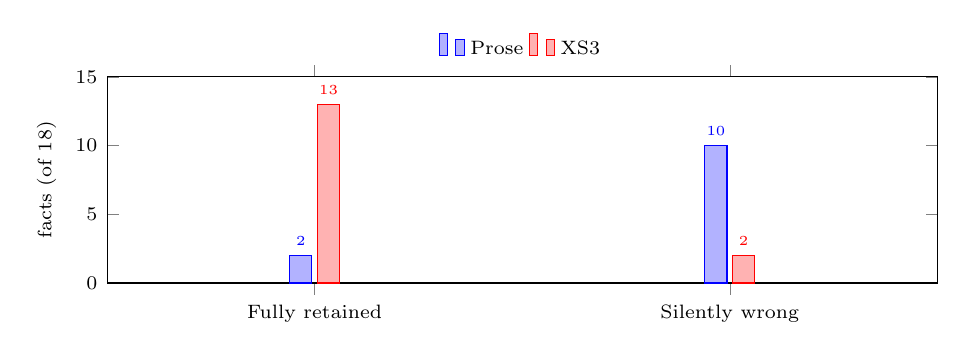
\begin{tikzpicture}
\begin{axis}[ybar, width=\columnwidth, height=4.2cm, font=\scriptsize,
  bar width=8pt, ymin=0, ymax=15, ylabel={facts (of 18)},
  symbolic x coords={Fully retained, Silently wrong}, xtick=data,
  legend style={at={(0.5,1.03)}, anchor=south, legend columns=2, draw=none},
  enlarge x limits=0.5, nodes near coords,
  every node near coord/.append style={font=\tiny}]
\addplot coordinates {(Fully retained,2) (Silently wrong,10)};
\addplot coordinates {(Fully retained,13) (Silently wrong,2)};
\legend{Prose, XS3}
\end{axis}
\end{tikzpicture}
\caption{Budgeted compaction (Study~S7). Prose retains few facts and silently
corrupts many; XS3 retains most and, when it sheds, omits whole edges rather than
corrupting what it keeps.}
\label{fig:drift}
\end{figure}

The counts matter less than the \emph{failure mode}. Prose failed by silent
corruption: ``desugars to \code{[s p o] mark not}'' became ``negates
\code{[s p o]}''; ``read correctly in \emph{blind} tests'' became ``verified'';
a rate qualifier was dropped while its fact was kept. Ten facts read plausibly
and were wrong. XS3 failed by omission: it dropped whole edges (which a reader
can detect as gaps), and what it retained stayed exact. For state that must be
trusted downstream, a missing fact is recoverable while a silently wrong fact is
not.

We note two honest limits. First, this is a fidelity result, not a compression
result: on already-terse fact lists XS3 is not smaller than prose (its
edge granularity can cost more tokens); the large token reductions XS3 achieves
elsewhere come from re-representing \emph{verbose} prose, not from compacting
terse state. Second, the advantage requires the stack-and-dedup instruction; told
to ``rewrite concisely,'' a model paraphrases XS3 too and drifts like prose.

\subsection{Edge aging and generational compaction}

\begin{figure}[t]
\centering
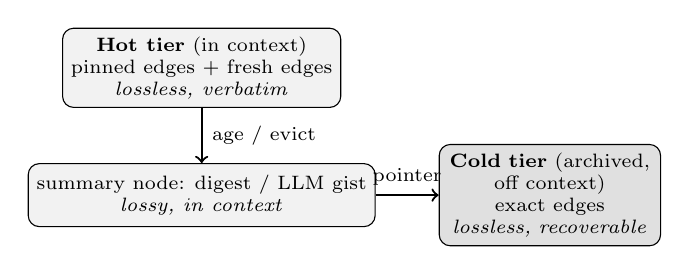
\begin{tikzpicture}[font=\scriptsize,
  box/.style={draw, rounded corners, align=center, inner sep=3pt, minimum height=8mm}]
\node[box, fill=black!5] (hot) {\textbf{Hot tier} (in context)\\ pinned edges + fresh edges\\ \emph{lossless, verbatim}};
\node[box, fill=black!5, below=7mm of hot] (sum) {summary node: digest / LLM gist\\ \emph{lossy, in context}};
\node[box, fill=black!12, right=8mm of sum, text width=2.6cm] (cold) {\textbf{Cold tier} (archived, off context)\\ exact edges\\ \emph{lossless, recoverable}};
\draw[->,thick] (hot) -- node[right]{age / evict} (sum);
\draw[->,thick] (sum) -- node[above]{pointer} (cold);
\end{tikzpicture}
\caption{Two-tier edge aging. Pinned and fresh edges stay verbatim in context; aged
ephemera collapse to an in-context summary that points to their byte-exact edges in a
cold archive, so the in-context state shrinks while nothing is lost.}
\label{fig:tier}
\end{figure}

Addressability enables policies that prose cannot express cleanly. Edges can be
timestamped (\code{@turn}) and evicted by recency; critical invariants (DOIs,
contracts) can be \emph{pinned} and exempted; and clusters of stale edges can be
reified into a single summary node that retains a pointer to what it replaced---a
generational, GC-like compaction. Each of these is a deterministic operation on
an edge set; none is expressible on prose without a rewrite, i.e., without
risking the very corruption Table~\ref{tab:drift} measures. We implement a
deterministic prototype combining recency eviction, pinning, and generational
cluster-merge. Over a scripted twelve-turn session with five ephemera per turn it
keeps every pinned fact---DOIs, invariants, commit hashes---\emph{byte-exact},
bounds the live set to a fixed slot budget, and packs the sixty aged ephemera
into four summary nodes; the compacted state is $73\%$ smaller than the un-aged
history ($223$ vs.\ $836$ tokens) with zero loss of any pinned fact. The scheme
is therefore \emph{selectively lossy}: pinned facts are preserved byte-exact
while ephemeral detail is reduced to a digest, and the $73\%$ saving comes
entirely from discarding that detail---this is eviction, not lossless
compression. To keep the discarded detail \emph{recoverable}
rather than merely counted, we add a cold archive tier keyed by the summary node
(Fig.~\ref{fig:tier}): the exact edges are held off-context and returned
byte-exact on demand, so the in-context saving costs no permanent loss. A summary
node's in-context text may be the deterministic digest or an LLM-generated gist
of the sacrificed cluster; because that cluster is disposable by construction, a
lossy gist there cannot corrupt any surviving fact. The contrast with prose is
thus not that XS3 loses less but that it loses \emph{safely}: what it keeps stays
exact, what it drops is named, and the detail remains recoverable, whereas prose
under the same budget silently corrupts what it appears to keep.

Recency alone, however, is blind to importance. On a probe where the durable
facts were old and the disposable actions were fresh, a keep-the-freshest policy
would retain \emph{none} of the six critical facts, whereas an LLM asked to rank
salience retained \emph{all six}. This motivates a hybrid selection policy: the
LLM \emph{decides} what to demote---a ranking it does well---but a deterministic
step \emph{executes} the compaction, keeping survivors verbatim and letting the
LLM summarize only the sacrificed cluster. True invariants are hard-pinned, so a
mis-ranking can at worst pack a fact (recoverable via its pointer), never
silently corrupt it. A full eviction policy and its evaluation across workloads
remain future work.

\section{Related Work}
XS3 is closest in spirit to RDF and its reification, and to controlled natural
languages such as Attempto Controlled English, but it inverts their usual
priority: it optimizes for a pre-trained reader rather than a hand-written
grammar, and it treats the parser as secondary to spec-free comprehension. Its
exactness mechanism resembles canonical serialization and graph canonical-labeling
(e.g., Weisfeiler--Leman for blank nodes) rather than constrained decoding, which
enforces grammar at generation time. Work on knowledge-graph compression (HDT,
grammar-based methods) targets scale-driven redundancy; we deliberately do not
claim token compression as XS3's contribution, and our measurements show it is
not one on information-dense input.

\section{Limitations and Future Work}
XS3 trades raw logical expressiveness for a monotone-graph invariant: it has no
native disjunction or unrestricted universal quantification, and negation is
confined to a single edge. Auto-injecting XS3 formatting into a host's automatic
compaction is not currently possible in at least one widely used agent runtime,
whose pre-compaction hook can only allow or block, not shape, the summary; the
practical channel is an explicit, manual compaction instruction. Future work
includes a formal eviction/aging policy, a study of multi-agent hand-off fidelity,
and a larger, pre-registered comprehension benchmark across model families and
sizes.

\section{Conclusion}
XS3 is a notation in which one sentence is one graph edge, every document decodes
deterministically to a triple graph, and the glyphs are chosen so a
specification-free model reads them from prior knowledge alone. Its practical
payoff is not brevity but \emph{trust}: as accumulated agent state is compacted
and re-read, atomic edges survive exactly or vanish visibly, whereas prose
corrupts silently. We believe corruption-resistant, addressable state is the
right foundation for machine-to-machine memory, and XS3 is a small, testable step
toward it.

\section*{Availability}
The language card and the reference decoder are archived on Zenodo under concept
DOI \texttt{10.5281/zenodo.21425813}, which always resolves to the latest version.

\begin{thebibliography}{1}
\bibitem{rdf} G. Klyne and J. J. Carroll, ``Resource Description Framework (RDF):
Concepts and Abstract Syntax,'' W3C Recommendation, 2004.
\bibitem{ace} N. E. Fuchs, K. Kaljurand, and T. Kuhn, ``Attempto Controlled
English for Knowledge Representation,'' in \emph{Reasoning Web}, LNCS 5224,
Springer, 2008, pp.\ 104--124.
\bibitem{hdt} J. D. Fern\'andez, M. A. Mart\'inez-Prieto, C. Guti\'errez,
A. Polleres, and M. Arias, ``Binary RDF Representation for Publication and
Exchange (HDT),'' \emph{J. Web Semantics}, 2013.
\bibitem{wl} B. Weisfeiler and A. Leman, ``The reduction of a graph to canonical
form and the algebra which appears therein,'' \emph{Nauchno-Tech. Informatsia},
ser.\ 2, no.\ 9, pp.\ 12--16, 1968.
\bibitem{cd} L. Beurer-Kellner, M. Fischer, and M. Vechev, ``Guiding LLMs the
Right Way: Fast, Non-Invasive Constrained Generation,'' in \emph{Proc. ICML},
PMLR vol.\ 235, 2024.
\end{thebibliography}

\end{document}
